% !TeX program = xelatex
\documentclass[a4paper,10pt]{article}

% ============================================================================
% សន្លឹកកិច្ចការសិស្សបំពេញចន្លោះ ស-ខ្មៅ និងប្លង់ក្ដារខៀន/ចម្លើយគ្រូ (គ្មាន LCD / គ្មានកន្ត្រៃ)
% មេរៀនទី៥ (៤.១–៤.២)៖ ការដាក់ជាផលគុណកត្តាតាមកត្តារួម និងសមភាពសំខាន់ៗ — ត្រូវគ្នានឹង LS_Plan_ALG57.tex
% ============================================================================
\usepackage[a4paper, left=1.0cm, right=1.0cm, top=0.75cm, bottom=1.00cm, footskip=0.52cm]{geometry}
\usepackage{amsmath}
\usepackage{unicode-math}
\usepackage{fontspec}
\usepackage{array, colortbl}
\usepackage[table]{xcolor}
\usepackage{enumitem}
\usepackage{pifont}
\usepackage{fancyhdr}
\usepackage{lastpage}
\usepackage{tikz}
\usepackage[most]{tcolorbox}
\usetikzlibrary{calc, arrows.meta, decorations.pathreplacing, positioning, babel}

\makeatletter
\let\@expl@@@mark@update@singlecol@structures@@\relax
\makeatother

\providecommand{\NGSFindFonts}{%
  \IfFileExists{C:/Windows/Fonts/cambria.ttc}{%
    \def\NGSSysPath{C:/Windows/Fonts/}%
    \def\NGSUserPath{C:/Users/KIT/AppData/Local/Microsoft/Windows/Fonts/}%
  }{%
    \IfFileExists{./fonts/KhmerOSsiemreap.ttf}{\def\NGSSysPath{./fonts/}\def\NGSUserPath{./fonts/}}{%
    \IfFileExists{../fonts/KhmerOSsiemreap.ttf}{\def\NGSSysPath{../fonts/}\def\NGSUserPath{../fonts/}}{%
    \IfFileExists{../../fonts/KhmerOSsiemreap.ttf}{\def\NGSSysPath{../../fonts/}\def\NGSUserPath{../../fonts/}}{%
    \IfFileExists{../../../fonts/KhmerOSsiemreap.ttf}{\def\NGSSysPath{../../../fonts/}\def\NGSUserPath{../../../fonts/}}{%
    \IfFileExists{../../../../fonts/KhmerOSsiemreap.ttf}{\def\NGSSysPath{../../../../fonts/}\def\NGSUserPath{../../../../fonts/}}{%
    \IfFileExists{../../../../../fonts/KhmerOSsiemreap.ttf}{\def\NGSSysPath{../../../../../fonts/}\def\NGSUserPath{../../../../../fonts/}}{%
    \IfFileExists{../../../../../../fonts/KhmerOSsiemreap.ttf}{\def\NGSSysPath{../../../../../../fonts/}\def\NGSUserPath{../../../../../../fonts/}}{%
      \def\NGSSysPath{../../../../../../../fonts/}\def\NGSUserPath{../../../../../../../fonts/}%
    }}}}}}}%
  }%
}
\NGSFindFonts

\setmathfont[Path={\NGSSysPath}, FontIndex=1, Scale=1.02]{cambria.ttc}
\defaultfontfeatures{Ligatures=TeX}

\setmainfont[
  Path={\NGSUserPath}, Extension=.ttf, Script=Khmer,
  BoldFont={KhmerOSsiemreap}, BoldFeatures={FakeBold=1.8},
  ItalicFont={KhmerOSsiemreap}, ItalicFeatures={FakeSlant=0.25},
  BoldItalicFont={KhmerOSsiemreap}, BoldItalicFeatures={FakeBold=1.8, FakeSlant=0.25}
]{KhmerOSsiemreap}

\newfontfamily\muol[Path={\NGSUserPath}, Extension=.ttf, Script=Khmer]{KhmerOSmuollight}
\newfontfamily\TimesEn[Path={\NGSSysPath}, Extension=.ttf, BoldFont={timesbd}, ItalicFont={timesi}, BoldItalicFont={timesbi}]{times}
\newfontfamily\CalibriFont[Path={\NGSSysPath}, Extension=.ttf]{calibri}

\XeTeXlinebreaklocale "km"
\XeTeXlinebreakskip = 0pt plus 1pt minus 0.1pt

\definecolor{panelgray}{gray}{0.94}
\definecolor{headgray}{gray}{0.85}

\pagestyle{fancy}
\fancyhf{}
\renewcommand{\headrulewidth}{0pt}
\fancyfoot[L]{\fontsize{7.4pt}{9.5pt}\selectfont អនុវិទ្យាល័យព្រះក្រសាំង \en{|} គ្រូ៖ ហុក ប៊ុនថែន \en{|} មេរៀនទី៥ (៤.១–៤.២) កត្តារួមនិងសមភាពសំខាន់ៗ \en{|} ថ្ងៃសុក្រ ទី១១ ខែធ្នូ ឆ្នាំ២០២៦}
\fancyfoot[R]{\fontsize{7.8pt}{10pt}\selectfont ទំព័រ \en{\thepage\ / \pageref{LastPage}}}

\setlength{\parindent}{0pt}
\setlength{\parskip}{0pt}
\setlength{\tabcolsep}{4pt}

\newcommand{\en}[1]{{\TimesEn #1}}
\newcommand{\enbf}[1]{{\TimesEn\bfseries #1}}
\newcommand{\unit}[1]{\,\text{\en{#1}}}
\newcommand{\riel}{\,\text{៛}}
\newcommand{\cnum}[1]{\mbox{\fontsize{10pt}{12pt}\selectfont\ding{\numexpr181+#1\relax}}}
\newcommand{\chkbox}{\tikz[baseline=-0.15ex]\draw[black, line width=0.85pt, fill=white] (0,0) rectangle (0.24cm,0.24cm);}
\newcommand{\ansbox}[1][2.0cm]{\,\tikz[baseline=-0.65ex]\draw[black, line width=0.65pt, fill=white] (0,0) rectangle (#1, 0.42cm);\,}
\newcommand{\dotline}[1][2.2cm]{\makebox[#1]{\dotfill}}

\newcommand{\pagebanner}[2]{%
  \begin{tcolorbox}[
    enhanced, sharp corners, colback=headgray, colframe=black,
    boxrule=1.05pt, boxsep=1pt, top=2.5pt, bottom=2.5pt, left=6pt, right=6pt,
    after skip=3.5pt
  ]
    {\muol\fontsize{9.0pt}{13.2pt}\selectfont #1}\hfill{\fontsize{8.0pt}{11.2pt}\selectfont\textbf{#2}}
  \end{tcolorbox}%
}

\newcommand{\secstrip}[2]{%
  \vspace{3pt}%
  \begin{tcolorbox}[
    enhanced, sharp corners, colback=panelgray, colframe=black,
    boxrule=0.8pt, boxsep=0.8pt, top=2pt, bottom=2pt, left=5pt, right=5pt,
    after skip=3pt
  ]
    {\muol\fontsize{8.5pt}{12.2pt}\selectfont #1}\hfill{\fontsize{7.8pt}{10.8pt}\selectfont\textit{#2}}
  \end{tcolorbox}%
}

\newcolumntype{L}[1]{>{\raggedright\arraybackslash}p{#1}}
\newcolumntype{C}[1]{>{\centering\arraybackslash}p{#1}}

\begin{document}
\fontsize{9.5pt}{14.5pt}\selectfont

% ============================================================================
% ទំព័រទី ១៖ សន្លឹកកិច្ចការសិស្ស (ផ្នែកមុខ៖ E1 -> E2 -> E3)
% ============================================================================
\pagebanner{សន្លឹកកិច្ចការសិស្ស \enbf{(}៥\enbf{.}៤\enbf{.}១\enbf{--}៤\enbf{.}២ កត្តារួម និងសមភាពសំខាន់ៗ\enbf{)} \enbf{--} ផ្នែកមុខ}{ថ្នាក់ទី៨ \en{|} ទំ.៦៨--៧០}

\begin{tcolorbox}[
  enhanced, sharp corners, colback=white, colframe=black,
  boxrule=0.8pt, boxsep=1.5pt, top=3.5pt, bottom=3.5pt, left=5pt, right=5pt,
  after skip=4pt
]
  \fontsize{9.0pt}{13.0pt}\selectfont
  \textbf{ឈ្មោះសិស្ស៖} \dotline[4.3cm] \quad
  \textbf{សមាជិកក្រុម៖} \dotline[4.3cm] \quad
  \textbf{ថ្នាក់ទី៖} ៨\dotline[0.9cm] \quad
  \textbf{ក្រុមទី៖} \dotline[1.0cm]
\end{tcolorbox}

% --- E1 Engage ---
\secstrip{ផ្នែកទី ១ \enbf{(E1 - Engage)} ៖ បេសកកម្មអន្ទាក់បំបាត់តួ $-1$ ពេលចាប់កត្តារួម}{រយៈពេល ៣ នាទី (គូស \ding{51} ក្នុង \chkbox)}

\begin{tcolorbox}[
  enhanced, sharp corners, colback=white, colframe=black,
  boxrule=0.8pt, boxsep=2.5pt, top=4pt, bottom=4pt, left=6pt, right=6pt
]
  គេចង់ដាក់កន្សោម $M = 5x(x + 2) - (x + 2)$ ជាផលគុណកត្តា ។ ពេល $x = 1$ គេបាន $M = 5(3) - 3 = \mathbf{12}$ ។ តើអ្នកណាត្រូវ?\\[3pt]
  \chkbox\ \textbf{សិស្ស ក៖} $M = (x + 2)(5x)$ \qquad\qquad
  \chkbox\ \textbf{សិស្ស ខ៖} $M = 5x(x + 2) - 1\cdot(x + 2) = (x + 2)(5x - 1)$\\[3pt]
  $\bullet$ \textbf{តេស្តដោយ $x = 1$៖} កន្សោមសិស្ស ក ស្មើ $3\times 5 =$ \dotline[1.2cm]; \ ឯកន្សោមសិស្ស ខ ស្មើ $3\times 4 =$ \dotline[1.2cm] ។
\end{tcolorbox}

\vspace{3pt}

% --- E2 Explore ---
\secstrip{ផ្នែកទី ២ \enbf{(E2 - Explore)} ៖ កត្តារួមជាឯកធា/ទ្វេធា និងសមភាពសំខាន់ៗ (ទំ.៦៨--៧០)}{រយៈពេល ១១ នាទី}

\textbf{សកម្មភាព ១ (\en{E2-A} — ៥ នាទី)៖ ៤.១ ការដាក់ជាផលគុណកត្តាតាមកត្តារួម (ទំ.៦៨--៦៩)}

\begin{tcolorbox}[
  enhanced, sharp corners, colback=white, colframe=black,
  boxrule=0.8pt, boxsep=2.5pt, top=4pt, bottom=4pt, left=6pt, right=6pt
]
  $\bullet$ \textbf{១) កត្តារួមជាឯកធា (ទំ.៦៨)៖} $3x + 3y + 3z =$ \ansbox[3.2cm] \qquad $6a^2b - 9ab^2 =$ \ansbox[3.6cm]\\[3pt]
  $\bullet$ \textbf{២) កត្តារួមជាទ្វេធា (ទំ.៦៩)៖} $x\underline{(2b - 3)} + y\underline{(2b - 3)} =$ \ansbox[3.8cm]\\[3pt]
  $\bullet$ \textbf{៣) លំហាត់គំរូ (ទំ.៦៩)៖} $(3x + 2y)\underline{(x + 1)} - y\underline{(x + 1)} = (x + 1)(3x + 2y - y) =$ \ansbox[3.8cm]
\end{tcolorbox}

\vspace{4pt}
\textbf{សកម្មភាព ២ (\en{E2-B} — ៦ នាទី)៖ ៤.២ ការដាក់ជាផលគុណកត្តាដោយប្រើសមភាពសំខាន់ៗ (ទំ.៦៩--៧០)}

\begin{tcolorbox}[
  enhanced, sharp corners, colback=white, colframe=black,
  boxrule=0.8pt, boxsep=2.5pt, top=4pt, bottom=4pt, left=6pt, right=6pt
]
  $\bullet$ \textbf{១) រូបមន្ត $(a \pm b)^2$ (ទំ.៦៩--៧០)៖} $4a^2 + 12a + 9 = (2a)^2 + 2(2a)(3) + 3^2 =$ \ansbox[3.2cm]\\[3pt]
  \hspace*{0.3cm}ខ) $\dfrac{x^2}{4} - 4x + 16 =$ \ansbox[2.45cm] \quad គំរូទី១៖ $x^2 + 10x + 25 =$ \ansbox[2.25cm] \quad $x^2 - 20x + 100 =$ \ansbox[2.35cm]\\[3pt]
  $\bullet$ \textbf{២) រូបមន្ត $a^2 - b^2$ និង $a^3 \pm b^3$ (ទំ.៧០, ៧៤)៖} $a^2 - 25 =$ \ansbox[3.2cm] \qquad $8x^3 + y^3 =$ \ansbox[4.4cm]\\[3pt]
  \hspace*{0.3cm}ខ) $27y^3 - 64 = (3y)^3 - 4^3 =$ \ansbox[4.8cm]
\end{tcolorbox}

\vfill

% --- E3 Explain ---
\secstrip{ផ្នែកទី ៣ \enbf{(E3 - Explain)} ៖ រូបមន្តបញ្ច្រាសទាំង ៥ និងធនាគារហេតុផល \enbf{B\&W}}{រយៈពេល ៦ នាទី}

\begin{tcolorbox}[
  enhanced, sharp corners, colback=white, colframe=black,
  boxrule=0.85pt, boxsep=2.5pt, top=4pt, bottom=4pt, left=6pt, right=6pt
]
  $\bullet$ \textbf{១) កត្តារួម៖} $ku \pm kv =$ \ansbox[2.8cm] \qquad\qquad \textbf{២) ការេទ្វេធា៖} $a^2 \pm 2ab + b^2 =$ \ansbox[3.0cm]\\[4pt]
  $\bullet$ \textbf{៣) ផលដកការេ៖} $a^2 - b^2 =$ \ansbox[3.4cm] \qquad \textbf{៤) ផលបូក/ដកគូប៖} $a^3 \mp b^3 = (a \mp b)($\dotline[2.4cm]$)$\\[4pt]
  \tikz\draw[black, dashed, line width=0.6pt] (0,0) -- (\linewidth,0);\\[3pt]
  \fontsize{8.8pt}{13.0pt}\selectfont
  \textbf{ធនាគារហេតុផល (\en{Warrant Bank})៖} \quad
  \cnum{1} ចាប់កត្តារួមធំបំផុតមុនគេជានិច្ច \quad
  \cnum{2} ចាប់តួទាំងមូលចេញ ត្រូវរក្សាមេគុណ $\pm 1$\\
  \cnum{3} ផ្ទៀងតួកណ្ដាលពិតជាស្មើ $\pm 2ab$ \quad
  \cnum{4} ផលបូកពីរការេ $a^2 + b^2$ មិនអាចដាក់ជាកត្តាក្នុង $\mathbb{R}$ បានទេ
\end{tcolorbox}

% ============================================================================
% ទំព័រទី ២៖ សន្លឹកកិច្ចការសិស្ស (ផ្នែកខាងខ្នង៖ E4 -> E5 -> កិច្ចការផ្ទះ)
% ============================================================================
\clearpage
\pagebanner{សន្លឹកកិច្ចការសិស្ស \enbf{(}៥\enbf{.}៤\enbf{.}១\enbf{--}៤\enbf{.}២ កត្តារួម និងសមភាពសំខាន់ៗ\enbf{)} \enbf{--} ផ្នែកខ្នង}{ថ្នាក់ទី៨ \en{|} ទំ.៧០, ៧៣--៧៤}

% --- E4 Elaborate ---
\secstrip{ផ្នែកទី ៤ \enbf{(E4 - Elaborate)} ៖ លំហាត់គំរូកត្តារួមរួមបញ្ចូលសមភាពសំខាន់ៗ (ទំ.៧០, ៧៤)}{រយៈពេល ១០ នាទី}

\begin{tcolorbox}[
  enhanced, sharp corners, colback=white, colframe=black,
  boxrule=0.8pt, boxsep=2.5pt, top=4pt, bottom=4pt, left=6pt, right=6pt
]
  \textbf{១) ចាប់កត្តារួមមុន រួចប្រើសមភាពសំខាន់ៗ (ទំ.៧០ និង ទំ.៧៤ \en{\#13} ច)៖}\\[3pt]
  \hspace*{0.3cm}$\bullet$ $4x^2 - 16xy + 16y^2 = 4(x^2 - 4xy + 4y^2) =$ \ansbox[3.8cm]\\[3pt]
  \hspace*{0.3cm}$\bullet$ $2m^2 + \sqrt{2}mn + \dfrac{n^2}{4} =$ \ansbox[3.8cm] \qquad
  $\bullet$ $5x^3 - 80x = 5x(x^2 - 16) =$ \ansbox[4.2cm]\\[4pt]
  \textbf{២) លំហាត់គំរូផលដកគូប និងផលបូកគូប (ទំ.៧០)៖}\\[3pt]
  \hspace*{0.3cm}$\bullet$ $x^3 - 27 =$ \ansbox[4.6cm] \qquad\qquad
  $\bullet$ $8a^3 + 1 =$ \ansbox[4.8cm]\\[4pt]
  \textbf{ឆ្លុះបញ្ចាំង (\en{EIA Looking-Back})៖} ហេតុអ្វី $x^2 + 9$ មិនអាចដាក់ជាកត្តា $(x+3)^2$ ឬ $(x-3)(x+3)$ បាន? \dotline[3.4cm] ។
\end{tcolorbox}

\vspace{4pt}

% --- E5 Evaluate ---
\secstrip{ផ្នែកទី ៥ \enbf{(E5 - Evaluate)} ៖ ប្រតិបត្តិ (ទំ.៧០, ៧៣--៧៤) សំណួរវិនិច្ឆ័យ \enbf{A--D} និងសំបុត្រចេញ}{រយៈពេល ១០ នាទី}

\begin{tcolorbox}[
  enhanced, sharp corners, colback=white, colframe=black,
  boxrule=0.8pt, boxsep=2.5pt, top=4pt, bottom=4pt, left=6pt, right=6pt
]
  \textbf{១) ប្រតិបត្តិជាក្រុម (ទំ.៧០ និង ទំ.៧៣--៧៤)៖}\\[3pt]
  \hspace*{0.3cm}$\bullet$ ទំ.៧០ (ក)៖ $x^2 - 8x + 16 =$ \ansbox[3.2cm] \qquad\qquad
  ទំ.៧០ (គ)៖ $n^2 - 12n + 36 =$ \ansbox[3.2cm]\\[3pt]
  \hspace*{0.3cm}$\bullet$ \en{\#11} ឃ៖ $x(4x - 8y) + y(x - 2y) =$ \ansbox[3.8cm] \qquad
  \en{\#13} ឃ៖ $x^2 - 4y^2 =$ \ansbox[3.4cm]\\[4pt]
  \textbf{២) បិទបេសកកម្ម \en{E1}៖} សិស្ស \dotline[1.1cm] ត្រឹមត្រូវ ព្រោះ $5x(x+2) - 1\cdot(x+2) =$ \ansbox[3.8cm] ។
\end{tcolorbox}

\vspace{4pt}

\begin{tcolorbox}[
  enhanced, sharp corners, colback=white, colframe=black,
  boxrule=0.85pt, boxsep=2.5pt, top=4pt, bottom=4pt, left=6pt, right=6pt
]
  \textbf{៣) សំណួរវិនិច្ឆ័យ \en{A--D} (ដាក់ $3x^2 - 12$ ជាផលគុណកត្តាឱ្យអស់លទ្ធភាព — គូសរង្វង់ រួចលើកម្រាមដៃ ១--៤)៖}\\[3pt]
  \textbf{\en{A.}} $3(x^2 - 4)$ \qquad\quad
  \textbf{\en{B.}} $(3x - 6)(x + 2)$ \qquad\quad
  \textbf{\en{C.}} $3(x - 2)(x + 2)$ \qquad\quad
  \textbf{\en{D.}} $3(x - 2)^2$\\[4pt]
  \tikz\draw[black, dashed, line width=0.6pt] (0,0) -- (\linewidth,0);\\[3pt]
  \textbf{៤) សំបុត្រចេញ ៦០ វិនាទី (ទំ.៧៤ \en{\#13} ដ)៖} ដាក់ជាផលគុណកត្តា $(x + 1)^2 - 4 =$ \ansbox[3.8cm] ។
\end{tcolorbox}

\vfill

% --- Homework Box ---
\begin{tcolorbox}[
  enhanced, sharp corners, colback=panelgray, colframe=black,
  boxrule=0.9pt, boxsep=2.5pt, top=4pt, bottom=4pt, left=6pt, right=6pt
]
  {\muol\fontsize{8.8pt}{13pt}\selectfont កិច្ចការផ្ទះ \enbf{(}សៀវភៅគោល ទំ\enbf{.}៧០ និង ទំ\enbf{.}៧៣\enbf{--}៧៤ លេខ ១១\enbf{--}១៤\enbf{)}}\\[3pt]
  $\bullet$ \textbf{១) ប្រតិបត្តិទំ.៧០ (ខ) និង \en{\#11} ខ (ទំ.៧៣)៖} ដាក់ជាផលគុណកត្តា $y^2 + 10y + 25$ និង $(3a^2 - 12a) - 5(a - 4)$ ។\\[2pt]
  $\bullet$ \textbf{២) ទំ.៧៤ \en{\#12} ក, ខ; \en{\#13} ក, ង និង \en{\#14} ង៖} ដាក់ជាផលគុណកត្តា $(2x-3)(5x-1)-(2x-3)(x+1)$, $(7a-1)^2-(7a-1)(3a+2)$, $a^2 - 25$, $25x^2 - 16y^2$ និង $a^2c - 2acx + cx^2$ ។
\end{tcolorbox}

% ============================================================================
% ទំព័រទី ៣៖ ទំព័រគ្រូបង្រៀន — ប្លង់ក្ដារខៀន ៣ ផ្នែក (គ្មាន LCD) និងចម្លើយផ្ទៀងផ្ទាត់រហ័ស
% ============================================================================
\clearpage
\pagebanner{ទំព័រគ្រូបង្រៀន ៖ ប្លង់ក្ដារខៀន \enbf{(}គ្មាន \enbf{LCD)} និងចម្លើយផ្ទៀងផ្ទាត់រហ័ស}{៥.៤.១--៤.២ កត្តារួម និងសមភាពសំខាន់ៗ (\en{ALG57})}

\secstrip{១. គំរូប្លង់បែងចែកក្ដារខៀន ៣ ផ្នែក សម្រាប់ថ្នាក់រៀនគ្មាន \enbf{LCD}}{សម្រាប់គ្រូប្រើដីស/ហ្វឺត}

\begin{center}
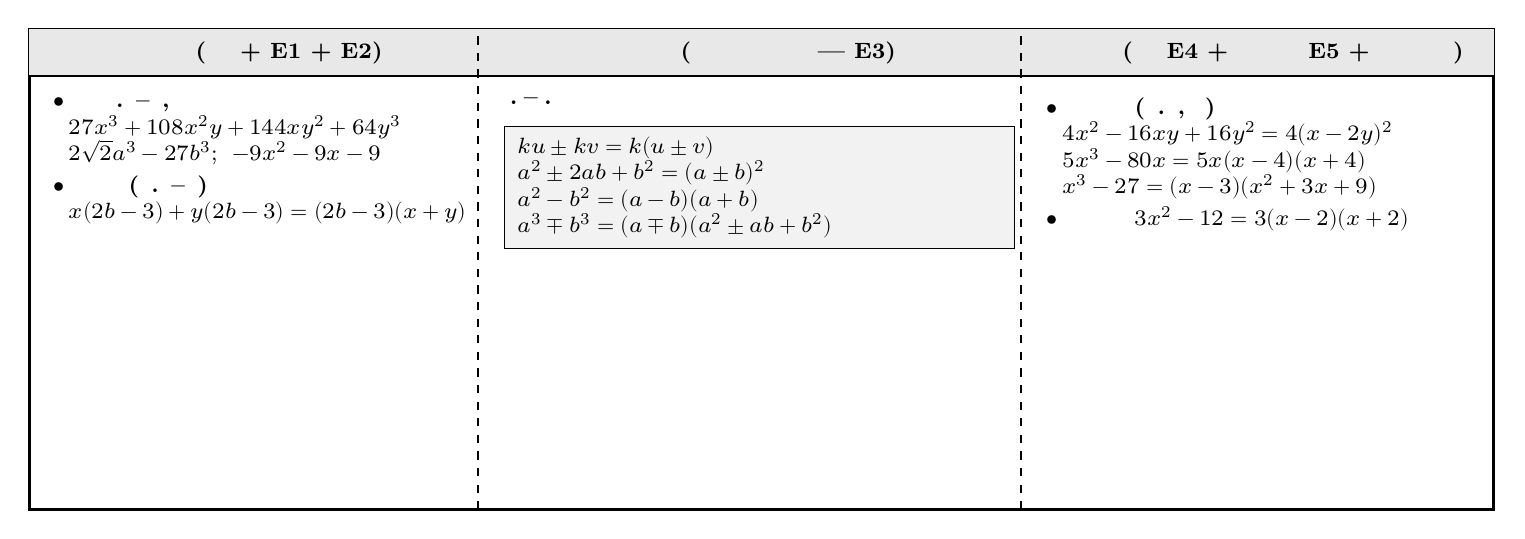
\begin{tikzpicture}[x=1cm, y=1cm, every node/.style={font=\footnotesize, text=black}]
  \draw[black, line width=1.1pt] (0,0) rectangle (18.6,6.1);
  \fill[gray!18] (0,5.50) rectangle (18.6,6.1);
  \draw[black, line width=0.7pt] (0,5.50) -- (18.6,5.50);
  \draw[black, dashed, line width=0.75pt] (5.7,0) -- (5.7,6.1);
  \draw[black, dashed, line width=0.75pt] (12.6,0) -- (12.6,6.1);

  \node at (2.85,5.80) {\textbf{ផ្នែកឆ្វេង (កំណែ + \en{E1} + \en{E2})}};
  \node at (9.15,5.80) {\textbf{ផ្នែកកណ្ដាល (ខ្លឹមសារគោលរក្សាទុក — \en{E3})}};
  \node at (15.60,5.80) {\textbf{ផ្នែកស្ដាំ (គំរូ \en{E4} + ប្រតិបត្តិ \en{E5} + កិច្ចការផ្ទះ)}};

  % Left zone
  \node[anchor=north west, text width=5.3cm] at (0.18,5.35) {
    $\bullet$ \textbf{កំណែ ទំ.៦៦--៦៧, ៧៣៖}\\
    \hspace*{0.2cm}$27x^3+108x^2y+144xy^2+64y^3$\\
    \hspace*{0.2cm}$2\sqrt{2}a^3-27b^3$; \ $-9x^2-9x-9$\\[2pt]
    $\bullet$ \textbf{កត្តារួម (ទំ.៦៨--៦៩)៖}\\
    \hspace*{0.2cm}$x(2b-3)+y(2b-3)=(2b-3)(x+y)$
  };

  % Center zone
  \node[anchor=north west, text width=6.5cm] at (5.90,5.35) {
    {\muol\fontsize{8.2pt}{12pt}\selectfont ៤\enbf{.}១\enbf{--}៤\enbf{.}២ រូបមន្តដាក់ជាកត្តា}\\[3pt]
    \begin{tcolorbox}[enhanced, sharp corners, colback=gray!10, colframe=black, boxrule=0.6pt, boxsep=1.5pt, left=3pt, right=3pt, top=2pt, bottom=2pt]
      $ku \pm kv = k(u \pm v)$\\
      $a^2 \pm 2ab + b^2 = (a \pm b)^2$\\
      $a^2 - b^2 = (a - b)(a + b)$\\
      $a^3 \mp b^3 = (a \mp b)(a^2 \pm ab + b^2)$
    \end{tcolorbox}
  };

  % Right zone
  \node[anchor=north west, text width=5.6cm] at (12.80,5.35) {
    $\bullet$ \textbf{លំហាត់គំរូ (ទំ.៧០, ៧៤)៖}\\
    \hspace*{0.2cm}$4x^2-16xy+16y^2 = 4(x-2y)^2$\\
    \hspace*{0.2cm}$5x^3-80x = 5x(x-4)(x+4)$\\
    \hspace*{0.2cm}$x^3-27 = (x-3)(x^2+3x+9)$\\[2pt]
    $\bullet$ \textbf{វិនិច្ឆ័យ៖} $3x^2-12 = 3(x-2)(x+2)$
  };
\end{tikzpicture}
\end{center}

\secstrip{២. ចម្លើយផ្ទៀងផ្ទាត់រហ័សសម្រាប់សន្លឹកកិច្ចការសិស្ស \enbf{(}ទំព័រ ១ និង ទំព័រ ២\enbf{)}}{\en{Answer Key}}

\begin{tcolorbox}[
  enhanced, sharp corners, colback=white, colframe=black,
  boxrule=0.8pt, boxsep=2.5pt, top=4pt, bottom=4pt, left=6pt, right=6pt
]
  $\bullet$ \textbf{ផ្នែក \en{E1}៖} សិស្ស ខ ត្រឹមត្រូវ $(x+2)(5x-1)$ ព្រោះពេល $x=1$ បាន $3\times 4 = 12$ (ឯសិស្ស ក បាន $15 \neq 12$) ។\\[2pt]
  $\bullet$ \textbf{ផ្នែក \en{E2}៖} សកម្មភាព ១៖ $3(x+y+z)$; $3ab(2a-3b)$; $(2b-3)(x+y)$; $(x+1)(3x+y)$ ។ សកម្មភាព ២៖ $(2a+3)^2$; $\left(\frac{x}{2}-4\right)^2$; $(x+5)^2$; $(x-10)^2$; $(a-5)(a+5)$; $(2x+y)(4x^2-2xy+y^2)$; $(3y-4)(9y^2+12y+16)$ ។\\[2pt]
  $\bullet$ \textbf{ផ្នែក \en{E4}៖} ១) $4(x-2y)^2$; $\left(\sqrt{2}m+\frac{n}{2}\right)^2$; $5x(x-4)(x+4)$; ២) $(x-3)(x^2+3x+9)$; $(2a+1)(4a^2-2a+1)$ ។\\[2pt]
  $\bullet$ \textbf{ផ្នែក \en{E5}៖} ១) $(x-4)^2$; $(n-6)^2$; $(x-2y)(4x+y)$; $(x-2y)(x+2y)$; ២) សិស្ស ខ; ៣) \textbf{ជម្រើស \en{C}} ($3(x-2)(x+2)$); ៤) $(x-1)(x+3)$ ។
\end{tcolorbox}

\secstrip{៣. ចម្លើយលម្អិតនៃកិច្ចការផ្ទះ \enbf{(}សម្រាប់ផ្ទៀងនៅដើមម៉ោងបន្ទាប់ ៥\enbf{.}៤\enbf{.}៣\enbf{)}}{សៀវភៅគោល ទំ.៧០, ៧៣--៧៤}

\begin{tcolorbox}[
  enhanced, sharp corners, colback=white, colframe=black,
  boxrule=0.8pt, boxsep=2.5pt, top=4pt, bottom=4pt, left=6pt, right=6pt
]
  $\bullet$ \textbf{១) ទំ.៧០ (ខ) និង \en{\#11} ខ៖} $y^2 + 10y + 25 = \mathbf{(y + 5)^2}$; \quad $(3a^2 - 12a) - 5(a - 4) = 3a(a - 4) - 5(a - 4) = \mathbf{(a - 4)(3a - 5)}$ ។\\[2pt]
  $\bullet$ \textbf{២) ទំ.៧៤ \en{\#12, \#13, \#14}៖} \en{\#12} ក៖ $2(2x-3)(2x-1)$; \ \en{\#12} ខ៖ $(7a-1)(4a-3)$; \ \en{\#13} ក៖ $(a-5)(a+5)$; \ \en{\#13} ង៖ $(5x-4y)(5x+4y)$; \ \en{\#14} ង៖ $a^2c - 2acx + cx^2 = c(a^2 - 2ax + x^2) = \mathbf{c(a - x)^2}$ ។
\end{tcolorbox}

\end{document}
